\documentclass{cs-moi}
\usepackage{geometry}
\usepackage{graphicx}
\usepackage{hyperref}

\title{Projet Messagerie C}
\author{Wassim Ben Nacef - Nabil Bennacer - Max Chateau}
\date{Polytech Montpellier - IG 3} 

\begin{document}
\maketitle{}
\begin{center}
	
\includegraphics[width=0.3\linewidth]{logoPolytech.png}
\end{center}

\vspace{4pt}
    \hrule
\vspace{4pt}
  
\section{Introduction}
\textbf{BetterSkype} est un projet de messagerie en C fonctionnant avec un modèle Client - Serveur via le terminal. Le code du projet est accessible sur Github (cf : Partie Annexes)

\begin{figure}[h!]
    \centering
    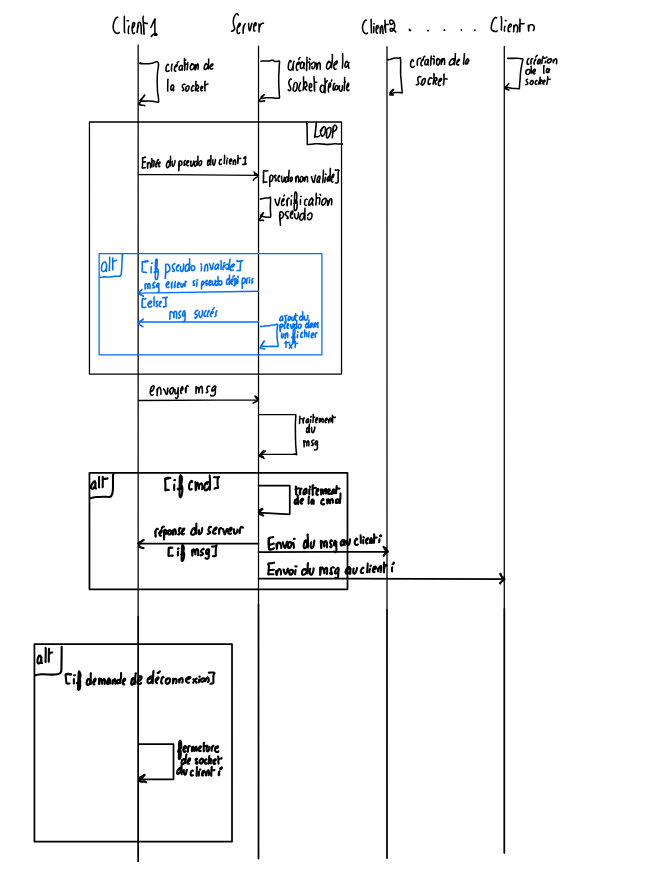
\includegraphics[width=0.5\linewidth]{seqGeneral.png}
    \caption{Diagramme de séquence du fonctionnement global du projet}
\end{figure}

\section{Développement}
\subsection{Problématiques}
Les différentes problématiques à gérer seront les choix de protocoles réseaux, ainsi que le choix des processus ou des threads.\\
Un autre problème sera la gestion de la communication entre le client et le serveur, ainsi que la gestion des messages (intégrité, connexion, etc...).\\
Enfin, un des derniers points sera la gestion des fichiers, ainsi que la gestion des utilisateurs (pseudos, adresses IP, etc...).

\subsection{Choix techniques}
En terme de communication nous avons fait le choix d'utiliser le protocole UDP pour les messages classiques, et TCP pour les envois de fichiers.

\begin{remarque}{Choix UDP + Processus}
     Ce choix s'explique d'une part pour des raisons de scalabilité et d'optimisation, dans la mesure ou ce protocole permet côté serveur de réceptionner des messages indépendamment de la personne qui l'envoie, sans consacrer un thread pour chaque utilisateur, ce qui permet de ne pas consommer trop de ressources à grande échelle, en plus de ne pas avoir à gérer pour $n$ utilisateurs, $n$ sémaphores côté serveur.\\
     Afin de garantir l'intégrité des messages, on va procéder à différentes vérifications (nombres de paquets reçu, accusé de réception...) lors de l'envoi et de la réception des paquets, ce qui permet de garder l'efficacité de l'UDP dans la majorité des cas de succès.\\
     On aura donc côté serveur, un processus qui s'occupera de gérer la reception des messages utilisateurs, ainsi qu'un autre processus qui gérera le renvoi des messages aux utilisateurs concernés. Idem côté client pour la communication avec le serveur. Celà nous permettra d'utiliser la communication interprocessus avec les signaux.
\end{remarque} 

\subsection{Solutions mises en places}
\subsubsection{Gestion des messages}
On va utiliser une structure de message qui va contenir les différentes propriétés afin de garantir la bonne transmission ainsi que l'intégrité des informations.\\
Lors de l'envoi on concatenera toutes les infos dans une chaine de caractères, qui seront séparées par des flags.

\begin{C}
    struct Message_S {
        char sender_ip[INET_ADDRSTRLEN];
        char dest_pseudo[PSEUDO_MAX];
        int  part_num;
        int  total_parts;
        char payload[BUFFER_MAX];
    };
    typedef struct Message_S Message;
\end{C}

\begin{figure}[h!]
    \centering
    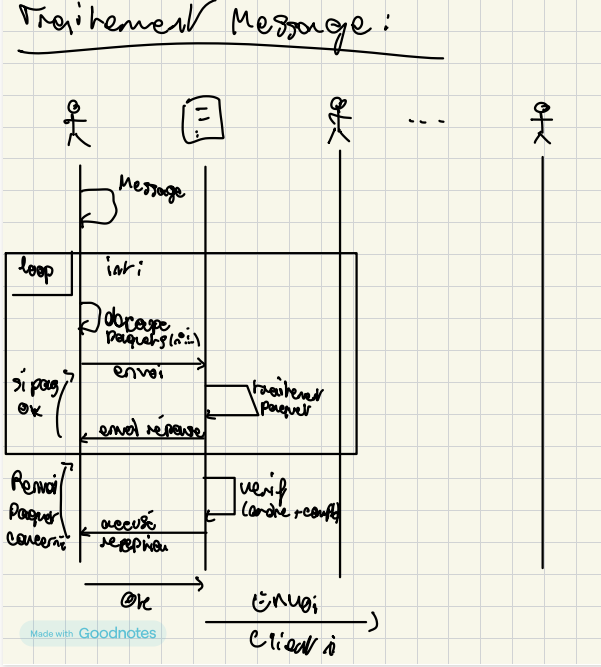
\includegraphics[width=0.7\linewidth]{diagMsg.png}
    \caption{Diagramme de séquence du fonctionnement des messages}
\end{figure}


\subsubsection{Makefile}
Le projet sera fournit avec un makefile qui permettra de compiler automatiquement tout les fichiers nécessaires au fonctionnement du projet, et de nettoyer les fichiers auxiliares via une simple commande.\\

\subsubsection{Gestion des utilisateurs}
On va utiliser un fichier csv pour stocker les utilisateurs, ainsi que leurs adresses IP associée.\\
Lors de la connexion d'un utilisateur, on va vérifier s'il n'est pas déjà connecté ailleurs, et si ce n'est pas le cas, on l'ajoute au fichier.\\
Lors de la déconnexion, on va supprimer l'utilisateur du fichier.\\

Pour gérer l'authentification, on stockera les couples (pseudo, mot de passe haché) dans un fichier csv, afin de vérifier l'existence des utilisateurs.\\
On integrera un système de hachage pour le mot de passe, afin de garantir la sécurité des données.\\

\subsubsection{Gestion des commandes}
On va utiliser un système de commandes, qui seront envoyées par le client au serveur, afin de lui indiquer ce qu'il doit faire.\\
Les commandes seront envoyées sous forme de message par l'utilisateur concerné.\\
Le serveur traitera les commandes en fonction de leur type et des autorisations, et renverra un accusé de réception à l'utilisateur concerné.\\

\subsubsection{Gestion des salons de discussions}
Un salon de discussion sera un dossier qui contiendra d'une part un ficheir csv avec les utilisateurs présents dans le salon, avec potentiellement des rôles (admin, utilisateur, etc...), ainsi qu'un fichier csv contenant l'historique des messages échangés dans le salon.\\

\subsubsection{Gestion des fichiers}
Pour la gestion des fichiers, on va utiliser le protocole TCP, afin de garantir l'intégrité des données.\\
Un utilisateur qui souhaite envoyer un fichier va d'abord envoyer un message de type fichier, qui contiendra le nom du fichier, ainsi que la taille du fichier.\\
Le serveur va ensuite créer une liaison TCP avec l'utilisateur, et lui demander d'envoyer le fichier.\\
On limitera le nombre d'utilisateurs pouvant envoyer un fichier en même temps, afin de ne pas saturer le serveur.\\

\newpage
\section{Organisation}
\subsection{Diagramme de Gantt}
\begin{figure}[h!]
    \centering
    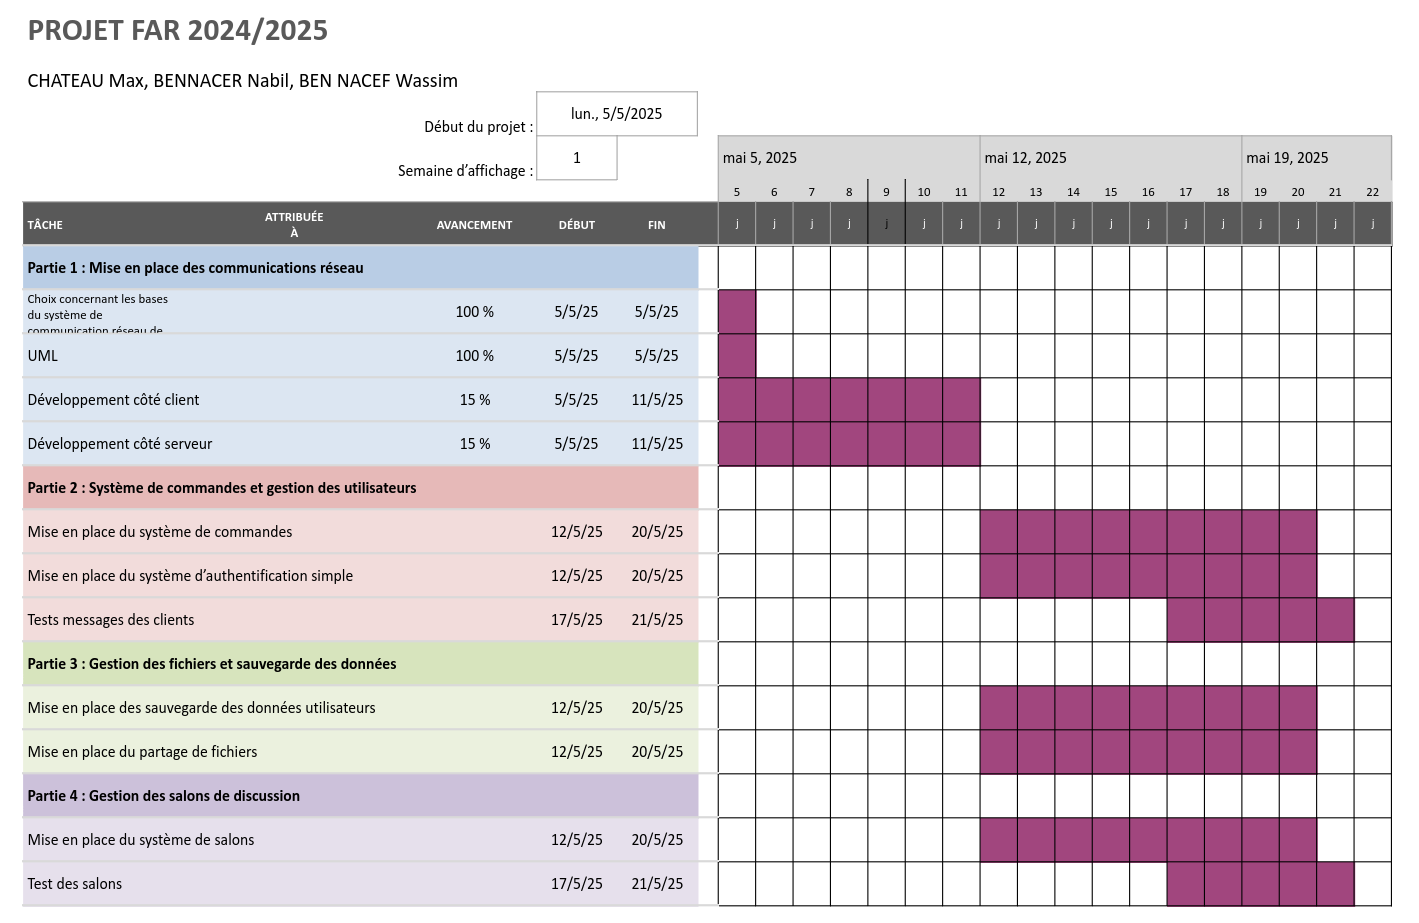
\includegraphics[width=0.95\linewidth]{Gantt.png}
    \caption{Diagramme de Gantt du projet}
\end{figure}

\subsection{Detail}
Pour une brève explication de l'organisation, on a decidé de se concentrer durant la première semaine sur la conception de la première partie afin d'être sûr de notre implémetation, et de ne pas perdre de temps sur des détails techniques par la suite.\\
On se concentrera ensuite sur les parties suivantes, à savoir la gestion des utilisateurs, des fichiers, et des salons de discussions lors de la deuxième semaine, en se répartissant une partie par personne.\\

\section{Avancement}
Actuellement, la première partie du projet est terminée, à savoir la gestion de la communication entre le client et le serveur.\\
On peut donc envoyer un message de type texte, et le serveur est capable d'interpréter toutes les informations contenues dans celui-ci, ainsi que de renvoyer un accusé de réception à l'utilisitateur concerné.\\

On a également mis en place un makefile qui permet de compiler le projet.


\section{Annexes}
\begin{itemize}
    \item \textbf{Github} : https://github.com/MaxbanCh/BetterSkype
\end{itemize}
\end{document}